\chapter{Test and Evaluation}
In this chapter, several performance tests will be done to the program developed for running CDSP. As there is no any other existing program developed for CDSP, the test results will not be compared to any others. The main purpose of these performance tests is to show the efficiency of the current implementation of CDSP so that it can be taken as a point of reference for future development.

The rest of the chapter will first describe the system environment that is used for the testing. Then tests results will be given for both Submit Protocol and Transmit Protocol separately. For each sub-protocol, two main kinds of test are done - latency test and scalability test. Finally a summary will conclude the testing result for both Submit and Transmit Protocol.

\section{Test Environment}
Following is a snapshot of the system environment used for the testing:\\

\noindent
\begin{tabular}{|l|p{0.6\textwidth}|}
 \hline
 Processor & Intel\textregistered \space Core\texttrademark \space i7-3610QM CPU @ 2.30GHz $\times$ 4 \\ \hline
 Installed Memory & 8 GB \\ \hline
 OS Platform & Ubuntu 12.04 LTS \\ \hline
 OS Type & 64-bit \\ \hline
 Network Interface & Loopback \\ \hline
 JRE Version & 1.7.0\textunderscore07 - b11 \\ \hline
\end{tabular}\\
\bigskip

\noindent
To eliminate the influence of various UI implementations, a UI called ``NullUserInterface" is used in the testing. In ``NullUserInterface", all parameters required from user input are all hard-coded thus it can be run automatically by only using commands. On the other hand, ``NullUserInterface" does not produce any output for user, it only outputs the testing results to the terminal so no extra computational resource will be used in dealing with outputs during the test.

\section{Submit Protocol}
\subsection{Latency Test}
The latency here refers to the total time cost for successfully running Submit Protocol once. It is defined as the time cost from the point that Courier initiates a connection to the point that Courier sends out the message 3 (a MAC as receipt confirmation). There are two reasons for defining the end point as Courier sending message 3, but not Alice receives message 3 : (1) It is very difficult to coordinate different times of two entities, especially in millisecond scale. (2) After Courier sends out message 3, it will leave immediately without caring whether the message will be received or not, and no further action of Courier depends on the arrival of message 3. Thus it is reasonable to define the sending of message 3 as the end of the Submit Protocol. 

The test programs contains running of two entities:
\begin{enumerate}
\item An Alice continuously listens to the port and is ready to start the Submit Protocol.
\item A Courier initiates the Submit Protocol, and once it sends out a message 3, it immediately creates another Courier and initiates the protocol with Alice again. This process repeats for 1000 times.
\end{enumerate}
The system records the time cost from the beginning of the program to Courier running the 100th, 200th, 300th,... 1000th times of the protocol respectively. The message content Alice sends is a 18 bytes string.

\begin{figure}[h!]
\centering
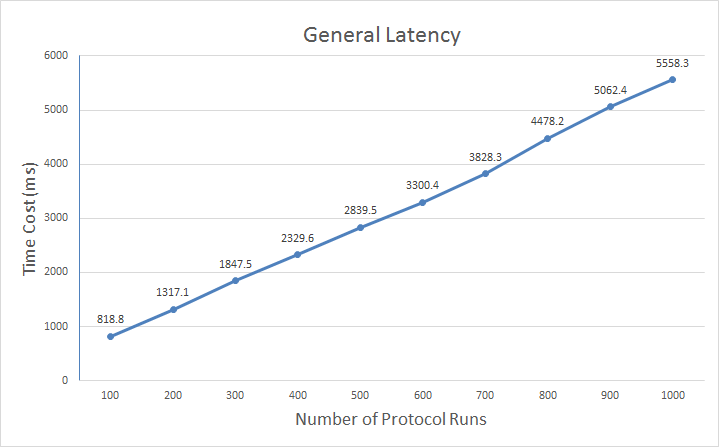
\includegraphics[width=0.7\textwidth,natwidth=719,natheight=447]{figures/latencysubmit.png}
\caption{General Latency Test of Submit Protocol}
\label{fig:latencysubmit}
\end{figure}

The test is done for totally 10 times and the final result is the average number of each testing result. Figure~\ref{fig:latencysubmit} shows the final result. Through the chart we can see the latency grows linearly with the number of communications - which is expected. And figure~\ref{fig:averagelatencysubmit} shows the average latency for every protocol run. The chart indicates that when the number of consecutive communication grows large, the average latency for each communication becomes stabilized around 5.5 milliseconds. In practice, there might be hundreds of entities within the system, a single message creator may send thousands of messages in a short period of time, and above result just proved that a single message creator is able to sequentially complete 1000 of message sending tasks around 5.5 seconds. This outcome is satisfying. 

\begin{figure}[h!]
\centering
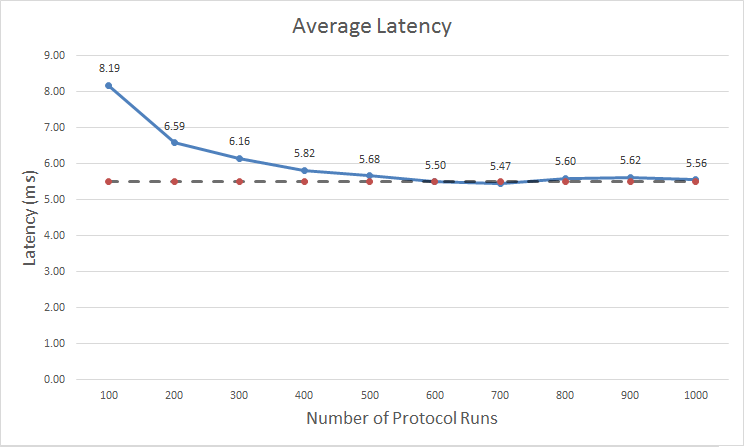
\includegraphics[width=0.7\textwidth,natwidth=744,natheight=447]{figures/averagelatencysubmit.png}
\caption{Average Latency of Submit Protocol}
\label{fig:averagelatencysubmit}
\end{figure}

\subsection{Scalability Test}
To thoroughly show the scalability of Submit Protocol, the performance of the protocol will be measured under two conditions - the growth of message size and the growth of communicating entities. Their methodologies and analysis results will be given separately below.

\subsubsection{Scale of Message Size}
In this test, it is expected to reveal how Submit Protocol will behave when the size of message to be sent increases.

The programs used are same with above latency tests - a normal message creator and a courier who repeatedly initiates Submit Protocol with the message creator.

The system records the latency of 1000th successful run of Submit Protocol with different sizes of messages. The message sizes are various from 1 byte to 10 KB. To make the test more convincing, we collect 5 data samples for every message size, and the result is plotted in a scatter chart figure~\ref{fig:messagesizesubmit}. The chart shows the total latencies for submitting 1000 times 1 Byte, 10 Bytes, 100 Bytes, 1 KB, 2 KB, 3KB, 4KB, 5KB and 10 KB messages respectively. It is shown that compare to the dramatical increasing extent of message size, the rise of latency is quite subtle - from around 5500 milliseconds to around 6200 milliseconds while message size is 10000 fold! Furthermore, following the trend line in the chart, it can also be observed that the grow trend of latency is linear which is ideal for the protocol.

\begin{figure}[h!]
\centering
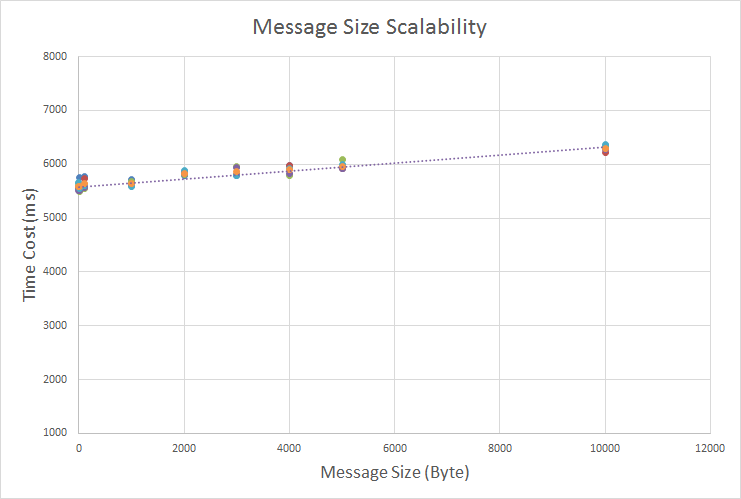
\includegraphics[width=0.7\textwidth,natwidth=741,natheight=499]{figures/messagesizesubmit.png}
\caption{Latency with Message Size for Submit Protocol}
\label{fig:messagesizesubmit}
\end{figure}

Using the same data sample, we can also calculate the relationship between the throughput and message size. We define the notion ``effective throughput" as the size of actual message content being sent per second. Namely, it does not count those extra bits which are the overhead for delivering the message. It represents the efficiency of the protocol in terms of delivering messages contents. Figure~\ref{fig:effectivethroughputsubmit} illustrates how the effective throughput of Submit Protocol changed when the message size increased. As the chart shows, the correlation between effective throughput and message size is linear, which is a good news because it means that the larger the messages are the more effective the protocol is. And when the message size increased to 10 KB, the effective throughput reaches nearly 1.6 MB/s. Of course, the effective throughput will not keep increasing infinitely, it will eventually hit the ceiling and restricted by the network throughput and capability of devices' available memory, however as 10 KB size is already considered very large for a single message, the efficiency at this level is good enough.

\begin{figure}[h!]
\centering
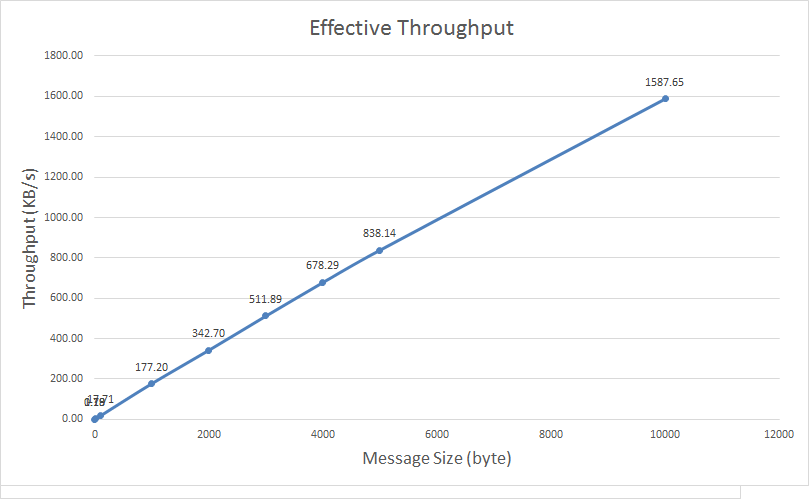
\includegraphics[width=0.7\textwidth,natwidth=809,natheight=499]{figures/effectivethroughputsubmit.png}
\caption{Effective Throughput with Message Size for Submit Protocol}
\label{fig:effectivethroughputsubmit}
\end{figure}

\subsubsection{Scale of Concurrent Communication}
In practice, it is highly probable that a single message creator will submit messages to several couriers simultaneously, this test reflects this scenario and aims to show the behaviour of Submit Protocol under the situation where concurrent communication is involved.

The testing program contains 3 entities:
\begin{enumerate}
\item An Alice continuously listens to the port and is ready to start the Submit Protocol.
\item A noisy Courier initiates the Submit Protocol with Alice, and once it sends out a message 3, it immediately creates another noisy Courier and initiates with Alice again. This process repeats for 100 times. It records the time cost for running 100 times of the protocol and yield the result.
\item Several silent Couriers initiate the Submit Protocol with Alice along with the noisy Courier. Same with noisy Courier, every silent Courier repeatedly initiates with Alice for 100 times, however, they do not record the time cost.
\end{enumerate}

Above settings is designed to extract the latency of a single communication when several communications are running simultaneously. During the test, the message size is 18 bytes and the number of active couriers are 1, 2, 3, 4, 5, 10, 20 respectively. Because such concurrent performance highly relies on the implementation of platform's scheduling mechanism, some extreme result may appear during the testing. Thus, to make the result more persuasive, every test is done for 7 times and the highest and lowest results are eliminated. The rest of results are plotted in scatter chart figure~\ref{fig:concurrentsubmit}. The trend line of the result appears to be polynomial in the order of 2. The reason that it is not linear is mainly because as the number of communication increases, the computational overhead for scheduling and switching processes also increases, so more concurrent communications it has, the more extra computation resource will be occupied.

\begin{figure}[h!]
\centering
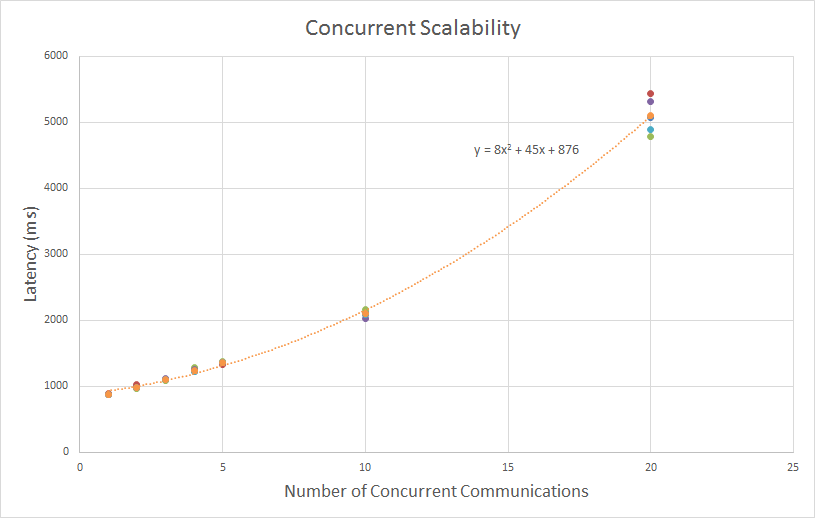
\includegraphics[width=0.7\textwidth,natwidth=815,natheight=518]{figures/concurrentsubmit.png}
\caption{Latency with Number of Concurrent Communications for Submit Protocol}
\label{fig:concurrentsubmit}
\end{figure}

Despite the polynomial growing trend, the protocol is still proved to be efficient under relatively small scale (less than 20 communications). The result shows that even when the message creator is communicating with 20 different couriers at the same time, the latency for running 100 times of protocol is still around 5 seconds (50 milliseconds for a single protocol run), considering the average latency for a single protocol run is 5.5 milliseconds (tested above), this result is fairly tolerable.

\pagebreak
\section{Transmit Protocol}
\subsection{Latency Test}
The definition of latency for Transmit Protocol is slightly different from Submit Protocol's. Referring to the protocol specification, Transmit Protocol requires only 2 messages, one forwarded from Courier to Bob, one replied from Bob to Courier. Here the latency is defined as the total time cost from the point that Courier initiates a connection, to the point that Courier receives the message 2 and finishes checking its validity.

Follow the same program settings of Submit Protocol, the latency tests for Transmit Protocol records the time cost for running 100, 200, 300, ..., 1000 times of the protocol. The message size is still 18 bytes.

\begin{figure}[h!]
\centering
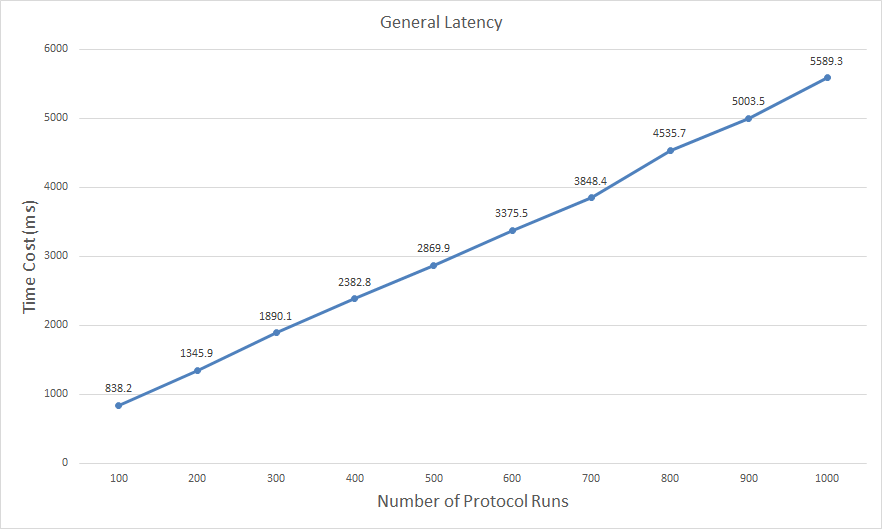
\includegraphics[width=0.7\textwidth,natwidth=882,natheight=529]{figures/latencytransmit.png}
\caption{General Latency Test of Transmit Protocol}
\label{fig:latencytransmit}
\end{figure}

Figure~\ref{fig:latencytransmit} shows the testing result. As expected, the outcome is quite similar to Submit Protocol, which appears to be linearly increasing. And even the average latency for each run of Transmit Protocol is same to Submit Protocol, which is given in figure~\ref{fig:averagelatencytransmit}. It can be observed that after doing Transmit Protocol many times, finally the average latency stabilized around 5.5 milliseconds. It proves the protocol is as efficient as Submit Protocol.

\begin{figure}[h!]
\centering
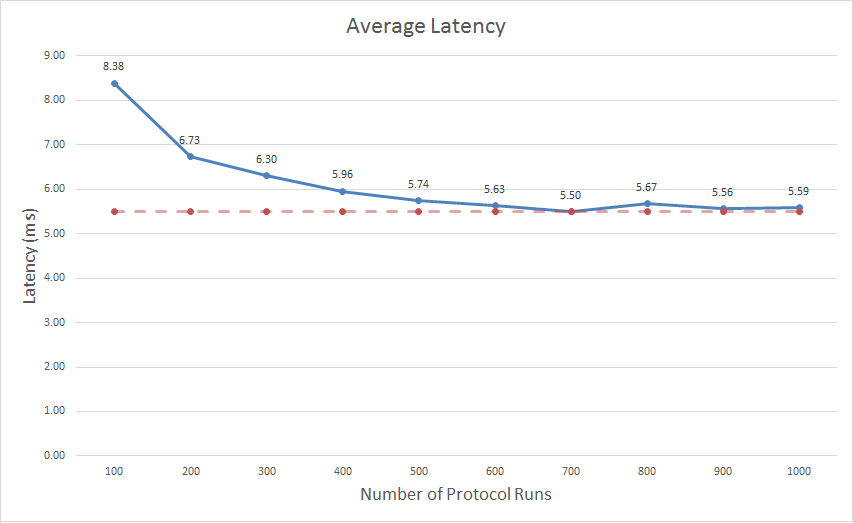
\includegraphics[width=0.7\textwidth,natwidth=853,natheight=523]{figures/averagelatencytransmit.png}
\caption{Average Latency of Transmit Protocol}
\label{fig:averagelatencytransmit}
\end{figure}

\subsection{Scalability Test}
In the scalability test of Transmit Protocol, besides testing under different scale of message size and number of concurrent communications, a new parameter is to be tested - number of messages. Their methodologies and analysis results will be given separately below.

\subsubsection{Scale of Message Size}
The methods and program settings used in this test is exactly the same with Submit Protocol, which is, a courier sends a message to Bob for 1000 times with different message size. The message sizes are 1 Byte, 10 Bytes, 100 Bytes, 1 KB, 2 KB, 3 KB, 4 KB, 5 KB and 10 KB respectively. The results are plotted in figure~\ref{fig:messagesizetransmit}, which indicates that the latency increase is fairly little comparing to the increase of message size. And it can be observed that the performance of Transmit Protocol when transmitting large messages is slightly better than Submit Protocol, it only takes 6 seconds to transmit a 10 KB message 1000 times, while it takes 6.2 seconds to submit it. 

\begin{figure}[h!]
\centering
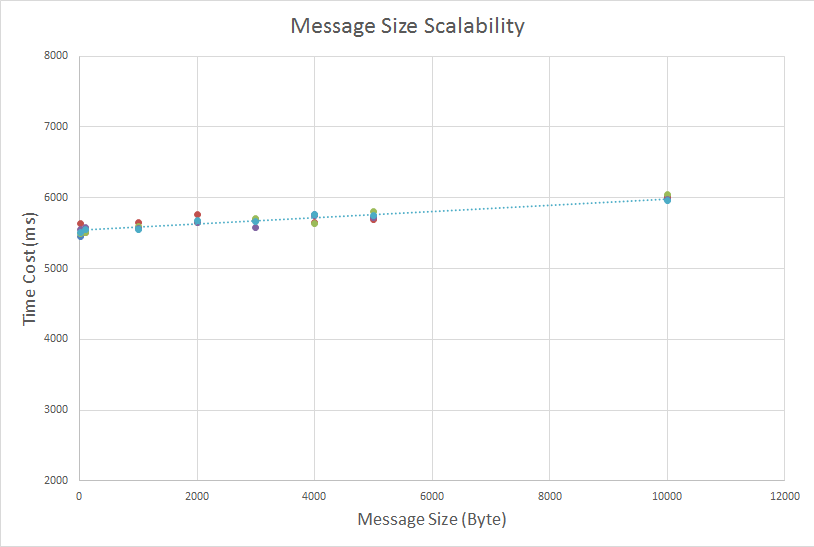
\includegraphics[width=0.7\textwidth,natwidth=814,natheight=547]{figures/messagesizetransmit.png}
\caption{Latency with Message Size for Transmit Protocol}
\label{fig:messagesizetransmit}
\end{figure}

The relationship between message size and effective throughput of Transmit Protocol is illustrated in figure~\ref{fig:effectivethroughputtransmit}. Similar to the Submit Protocol, the effective throughput has linear positive correlation with the message size. It means the larger the size of single message is, the more efficient of the protocol will be. And by observing figure~\ref{fig:effectivethroughputsubmit} and figure~\ref{fig:effectivethroughputtransmit}, we can conclude that overall, the efficiency of Transmit Protocol is slightly better than Submit Protocol because its latency is always less than Submit Protocol when they are tested under the same condition.

\begin{figure}[h!]
\centering
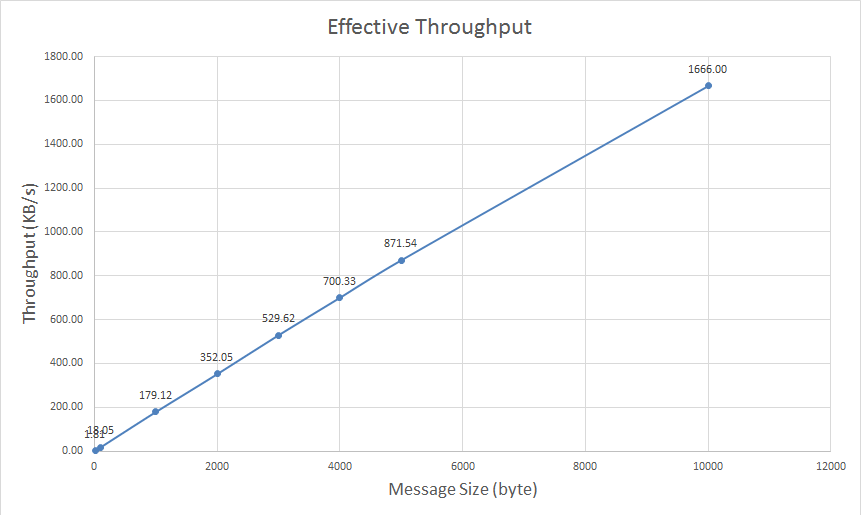
\includegraphics[width=0.7\textwidth,natwidth=861,natheight=515]{figures/effectivethroughputtransmit.png}
\caption{Effective Throughput with Message Size for Transmit Protocol}
\label{fig:effectivethroughputtransmit}
\end{figure}

\subsubsection{Scale of Concurrent Communication}
Same concurrency test is done to Transmit Protocol to reflect the practical scenario when a single message recipient (Bob) may receive messages from multiple couriers. The program settings are same to Submit Protocol: certain number of silent couriers keep communicating with Bob silently, while one noisy courier records the number of communication and yields the time cost. 

The testing result is shown in the figure~\ref{fig:concurrenttransmit}. The trend line of data samples is quite similar to the one of Submit Protocol, they both indicate a polynomial correlation. However, the growth rate of it in Transmit Protocol is much less than in Submit Protocol. We can find that when communicating with 20 couriers, Transmit Protocol takes only 3.2 seconds to complete 100 times of protocol, while Submit Protocol takes about 5 seconds. It means courier will be more efficient to transmit messages than to receive messages.

\begin{figure}[h!]
\centering
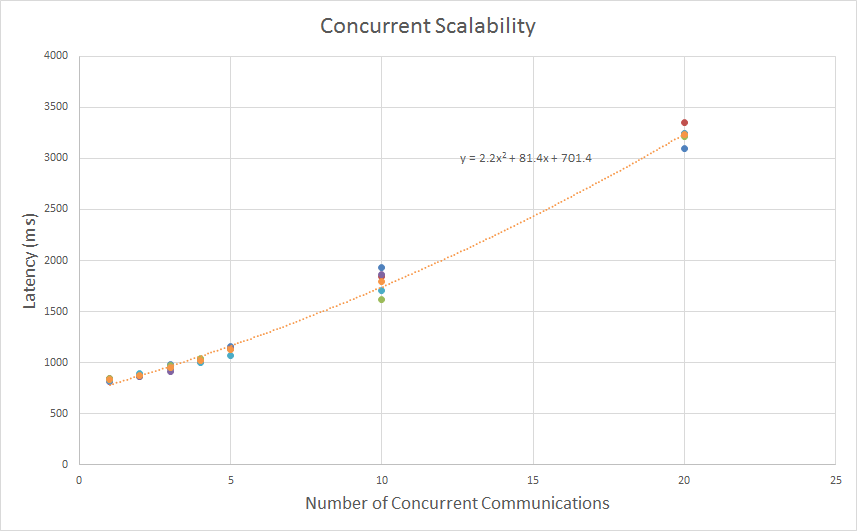
\includegraphics[width=0.7\textwidth,natwidth=857,natheight=531]{figures/concurrenttransmit.png}
\caption{Latency with Number of Concurrent Communications for Transmit Protocol}
\label{fig:concurrenttransmit}
\end{figure}

\subsubsection{Scale of Message Number}
This test simulates a common situation that a single Courier carries messages from several message creators and transmit it to the message recipient once for all. It is the most basic communication model in the system, so we are curious about how it performs in the actual implementation. Theoretically, the number of messages raises does not only lead to the increasing of message size, more extra checking processes are required as well. The test aims to find out how severe its influence will be.

This test measures the latency of total 100 Transmit Protocol runs with different number of messages transmitted. The number of messages are 1, 2, 3, 4, 5, 10, 20, and each message has size of 1 KB. Totally 5 tests are done and the average number of them is taken as the final outcome.

Figure~\ref{fig:messagenumbertransmit} shows the linear correlation of between number of messages and latency. It indicates that to sequentially complete 100 Transmit Protocols for a courier who carries 20 messages, it takes about 4 seconds in total, which means 40 milliseconds for every completion of the protocol. It is a great cost increase comparing to 5.5 ms, which is the average latency per protocol run. 

\begin{figure}[h!]
\centering
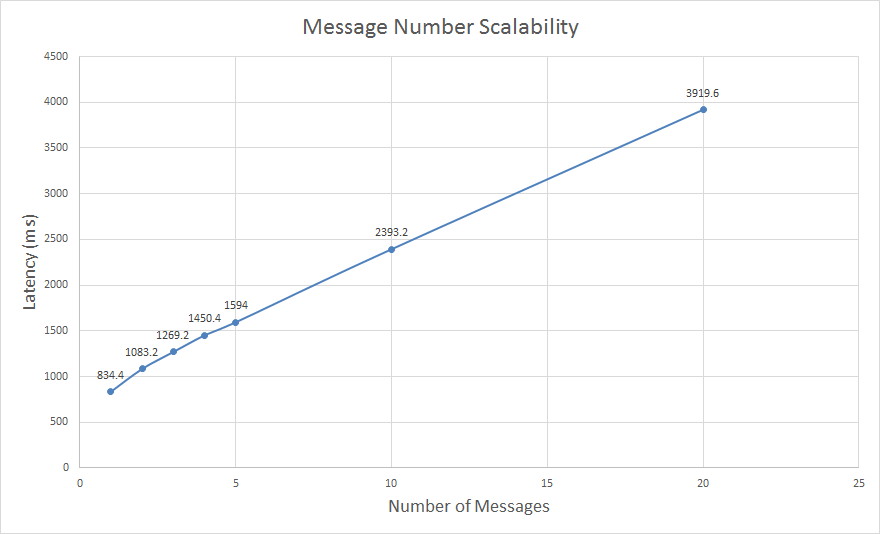
\includegraphics[width=0.7\textwidth,natwidth=880,natheight=534]{figures/messagenumbertransmit.png}
\caption{Latency with Number of Messages for Transmit Protocol}
\label{fig:messagenumbertransmit}
\end{figure}

Furthermore, the figure~\ref{fig:throughputcomparison} compares the efficiency difference between transmitting a large message as whole and chopping it into several pieces of smaller messages. The comparison takes several large size messages, and (1) transmits it as a whole, (2) transmits it as several 1 KB size smaller messages, and show their effective throughput respectively. The result conveyed by the figure is absolutely clear: no matter what the total message size is, transmitting it as a large message has nearly twice the throughput than chopping it up.

\begin{figure}[h!]
\centering
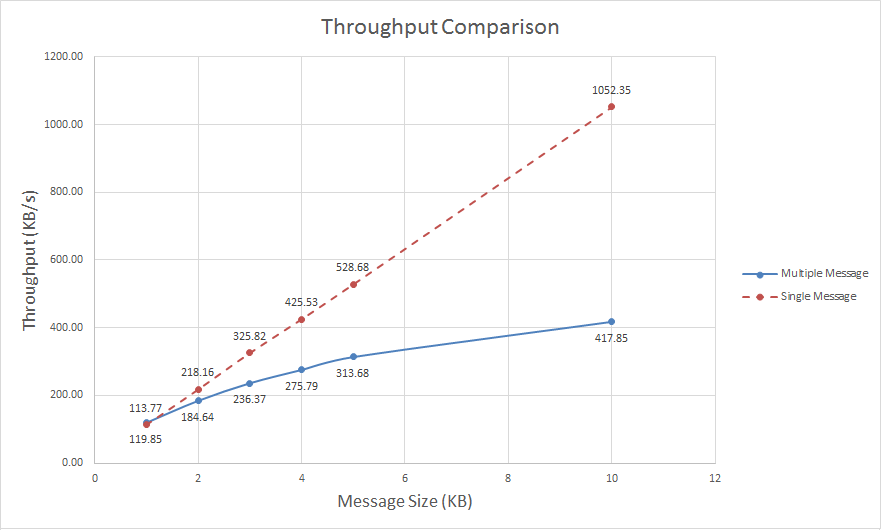
\includegraphics[width=0.7\textwidth,natwidth=881,natheight=530]{figures/throughputcomparison.png}
\caption{A Large Message or Several Small Messages?}
\label{fig:throughputcomparison}
\end{figure}

Conclusions drawn from both figure~\ref{fig:messagenumbertransmit} and figure~\ref{fig:throughputcomparison} indicate that transmitting large number of messages in a single Transmit Protocol is very time consuming. Thus when Alice sending a large message to Bob, it is recommended to send it as a whole for the efficiency concern.

\section{Summary}
In this chapter, mainly two kinds of tests are applied to both Submit Protocol and Transmit Protocol respectively - latency test and scalability test. Latency test evaluates the time cost for completing a protocol under a relatively low workload, while scalability test reveals the behaviour of both protocols when the system scale dramatically grows. The testing results prove that both Submit and Transmit Protocol are very efficient, every single run of protocol in low-workload situation takes only 5.5 milliseconds for both of the protocols. And in terms of scalability, both sub-protocols behave surprisingly the same. Firstly they are both not sensitive to the increasing of message sizes, and their latencies have polynomial correlation with the number of concurrent communications. Besides, through the analysis of relation between latency and number of message sizes, it has been emphasized that sending a large message as whole is far better than sending it as several pieces of smaller messages.